% Бүлэг 2

\chapter{Системийн шаардлага ба шинжилгээ} % Бүлгийн нэр
\label{Chapter2} % Энэ бүлэг рүү ишлэл хийх бол \ref{Chapter1} командыг ашигла 

\section{Системийн үйл ажиллагааны тухай дэлгэрэнгүй }
\qquad Агуулах нь байгууллагын бараа материал, түүхий эд, хангамжийн материал, үндсэн хөрөнгө зэрэг хөрөнгүүдийг татан авах, байршуулах, хадгалах, дамжуулах, зарлагадах зэрэгт зориулагдсан байр, байгууламж юм. Танай байгууллагын үйлдвэрлэл, борлуулалт, төлөвлөлтийн үйл ажиллагааг тасралтгүй байлгаж, улмаар үргүй зардал гаргахгүйн тулд Агуулахын төлөвлөлт зохион байгуулалтыг зөв зохистой, оновчтой явуулах шаардлагатай юм.

Агуулах нь захиалагч болон нийлүүлэгч хоёрын хооронд бүтээгдэхүүүнийг захиалагчдад хүлээлгэн өгөхтэй холбогдсон бүтгээгдэхүүний бөөгнөрүүлэн хуримтлуулах, бүртгэх, хадгалах, материал, түүхий эд, бэлэн бүтээгдэхүүнд харьцангуй бага нэмүү өртгийг бий болгодог. 

\section{Системийг ашиглах хэрэглэгчид}
\begin{itemize}
\item Агуулахын нягтлан
\item Админ

\end{itemize}
\section{Функционал шаардлага}

\qquad Энэхүү веб нь агуулахын нягтлан, админ, гэсэн 2-н оролцогчтой.
Нягтлан нь: Нягтлан нь агуулахын үйл ажиллагаа хариуцаж явуулах.
Админ: Бүх хуудсыг хянах, бүртгэлтэй хэрэглэгч болон вебийн ерөнхий мэдээллийг удирдах.

Нягтлангийн функциональ шаардлага:
\begin{enumerate}
	\item  Бараа, бүтээгдэхүүний үйл ажиллагааг удирдах
	\begin{enumerate}
		\item[1.1]  Дансны бүлгийг харах
		\item[1.2]  Дансны жагсаалтыг хэвлэх
		\item[1.3] Шинээр данс бүртгэх
	    \item[1.4]  Харилцагч бүртгэх
	    \item[1.5] Үндсэн хөрөнгө барааг бүртгэх (бүлэг, барааны код, нэр, хэмжих нэгж,  ангилал, тоо ширхэг, нэгж үнэ, бөөний үнэ, нийт үнэ).
	  	\item[1.10] Үндсэн хөрөнгө данслах.
	  	\item[1.13] Худалдан авалтын падаан хэвлэх. 
	  	\item[1.14] 	Худалдан авалтын буцаалт (огноо, байршил, баримтын дугаар, харилцагчын нэр )
	  	Бараа-барааны код, барааны нэр, тоо хэмжээ, нэгжийн өртөг, нэгжийн өртөг/НӨАТ/, дүн, НӨАТ, данс, буцаах тоо хэмжээ, дүн, буцаалтын дараах тоо хэмжээ.
	  	\item[1.15] Худалдан авалтын буцаалтын падаан хэвлэх.
	  	\item[1.16] Бараа материал борлуулалт хийх.
	  	\item[1.17] Борлуулалтын падаан хэвлэх.
	  	\item[1.18]	Борлуулалтын буцаалт хийх.
	  	\item[1.19]	Борлуулалтын буцаалтын падаан гаргана.
	  	\item[1.20] Тайлан гаргах.
	  	
	  	Бараа материалын үнийн өөрчлөлтийн тайлан
	  	
	  	Бараа материалын орлого зарлагын тайлан
	  	
	  	Бараа матераилын борлуулалтын тайлан
	  	
	  	Бараа материалын ашгийн тайлан
	  	
	  	Бараа материалын зарлага, зардлын тайлан
	  	
	  	Бараа материалын борлуулалт, худалдан авалтын тайлан
	  	
	  	Бүтээгдэхүүн өртгийн тооцооны тайлан
	  	
	  	Бараа материал зарцуулалтын тайлан
	  	
	  	Бараа материалын дэлгэрэнгүй тайлан
	  	\end{enumerate}
\end{enumerate}
Админы функциональ шаардлага:
\begin{enumerate}
	\item Хэрэглэгч бүртгэх
	\begin{enumerate}
		\item[1.1] Хэрэглэгчийн нэвтрэх нууц үг болон нэрийг бүртгэх.
		\item[1.2] Хэрэглэгч нэмэх, хасах, устгах.
	\end{enumerate}
	\item Бүх лавлахуудын бүртгэх
	\begin{enumerate}
		\item[2.1] Дансны бүлэг нэмэх, засах, устгах.
		\item[2.2] Данс нэмэх, засах устгах.

	\end{enumerate}
\end{enumerate}

\section{Функционал бус шаардлага}
\subsection{Гүйцэтгэлийн шаардлага}
\begin{enumerate}
	\item Өгөгдлийн сан ачааллах хугацаа нь хурдан шуурхай байх
	\item Хэрэглэгчдэд ойлгомжтой загвартай байх 
	\item Гүйцэтгэлийн хурд нь 3-5 секундэд багтан гардаг байх 
	Архитектурын хувьд үйлдлийн системийн орчинд хөгжүүлдэн
	
\end{enumerate}
\subsection{Аюулгүй байдлын шаардлага}
\begin{itemize}
	\item Бүртгэлийн хэсэг дээр хэрэглэгчийн нууц үгийг илүү нарийвчлалтайгаар аваагүйгээс тухайн хэрэглэгчдийн нууц үгийг ямар нэгэн гадны этгээд тааж цаашлаад тухайн хэрэглэгчийн, болон байгууллагын чухал чухал мэдээллүүд рүү халдах боломжтой. 
	\item Гадны ямар нэгэн халдлагаас болж сервер унах, ачааллаа даахаа болих. Үүнээс болж системийн үйл ажиллагаа зогсох магадлал өндөр юм.
\end{itemize}
\subsection{Хамгаалалт, нууцлалын шаардлага}
\begin{itemize}
	\item Системийн хэрэглэгч нууц үг, пасспорттой байх ёстой
	\item Дэлгэцэнд нууц үгийг харуулдаггүй байх ёстой
	\item Мөн ганц төхөөрөмжөөс нэвтрэх ёстой
	\item Сард нэг удаа паспортоо солих 
\end{itemize}
\subsection{Програм хангамжийн чанарын шаардлага}
\qquad Энэхүү систем нь дараах шаардлагуудыг илүү сайн хангаж байгаа юм. Үүнд:
\begin{itemize}
	\item Уян хатан байдал (хэрэглэгчийн шаардлага, санал хүсэлтэнд нийцүүлсэн байх.)
	\item Ашиглахад хялбар байдал (системийн зохиомж болон функцүүдийн хувьд бүхий л хүнд ойлгомжтой байна.) 
	\item Систем нэг зэрэг олон хандалт хүлээн авах чадвартай байх.
\end{itemize}
\section{Ашигласан технологи, техникийн шаардлага}
\subsection{Технологийн шаардлага}
\subsubsection{Програм ажиллах үйлдлийн системийн сонголт}
\qquad
Энэхүү систем нь вэб орчинд ажиллана. Тиймээс вэб үйл ажиллагааг дэмждэг бүхий л үйлдлийн системийн хувьд бүрэн ажиллах боломжтой. 
Програм ажиллах үйлдлийн системүүд: 
\begin{enumerate}
	\item Windows OS:Vista/7/8/10 
	\item Ubuntu OS: 10.04/10.10/11.04/11.10/12.04/12.10
	
\end{enumerate}
\subsubsection{Програм хөгжүүлэх хэлний сонголт}
\begin{enumerate}
	\item HTML5
	\item CSS
	\item JavaScript
	\item PHP
\end{enumerate}
\subsubsection{Програм хөгжүүлэх хэлний сонголт}
\begin{enumerate}
	\item HTML5
	\item CSS
	\item JavaScript
	\item PHP
\end{enumerate}

\subsubsection{Өгөгдлийн сангийн удирдах системийн сонголт}
\qquad
Энэхүү системийнхээ баазыг MySQL өгөгдлийн сан удирдах систем дээр хийж хөгжүүлэхээр болсон бөгөөд MySQL нь холбоост өгөгдлийн санг удирдах систем юм. 
\subsubsection{Баримт бичгийн боловсруулалтын системийн сонголт}
Бичиг баримт боловсруулалттай ажлын хувьд: 
\begin{itemize}
	\item MS Office Word 2016 
	\item Visual Paradigm 2015 
	\item MS Office Visio 2016
	\item Photoshop CS6 
	\item www.draw.io 
\end{itemize}
Танилцуулах програмын хувьд: 
\begin{itemize}
	\item MS Powerpoint 
\end{itemize}
%-----------------------------------------------------------------------   
\vspace*{1.5in} 
\subsection{Техникийн шаардлага}
\subsubsection{Оролт гаралтын төхөөрөмжүүдийн шаардлага}
\begin{longtable}{| p{0.7cm} | p{4cm} | p{3.5cm} | p{3.3cm} |}
	\hline
	\textbf{№} & \textbf{Төхөөрөмж} & \textbf{Төрөл} & \textbf{Шаардлага}\\
	\hline
	1 & \begin{center}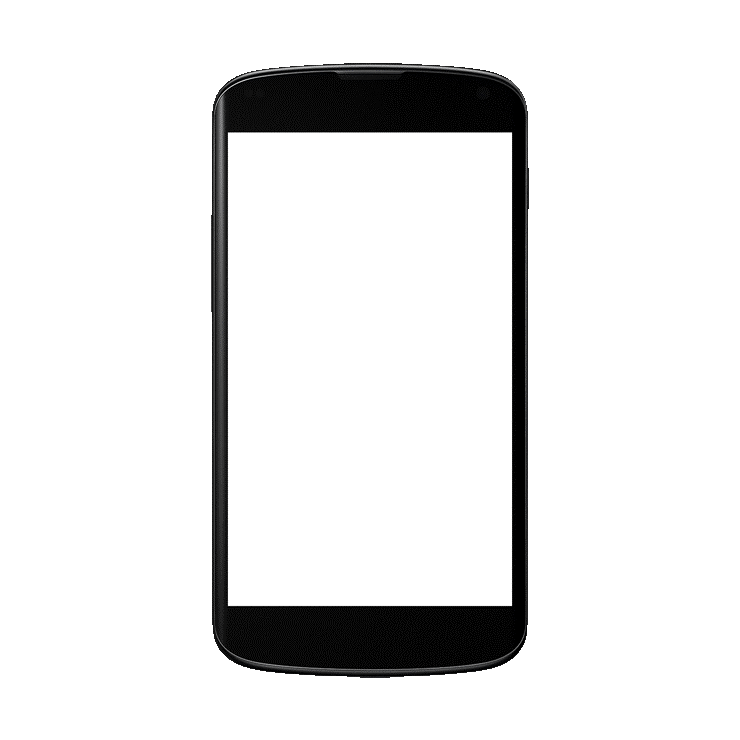
\includegraphics[width=2cm]{Diagrams/icon1} \end{center}& Мэдрэх & Энгийн  \\
	\hline
	2 & \begin{center}
\includegraphics[width=2cm]{Diagrams/icon2} \end{center} & Оролт & Энгийн \\
	\hline
	3 & \begin{center}
\includegraphics[width=2cm]{Diagrams/icon3} \end{center} & Гаралт & Дурын  \\
	\hline
	4 & \begin{center}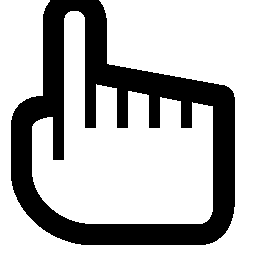
\includegraphics[width=2cm]{Diagrams/icon4} \end{center} & Заах & Дурын \\
	\hline
	\caption[Оролт гаралтын төхөөрөмжүүдийн шаардлага]{Оролт гаралтын төхөөрөмжүүдийн шаардлага}
	
\end{longtable}
\vspace*{1.5in}
\section{Юзкейс диаграм}
\begin{figure}[!h]
	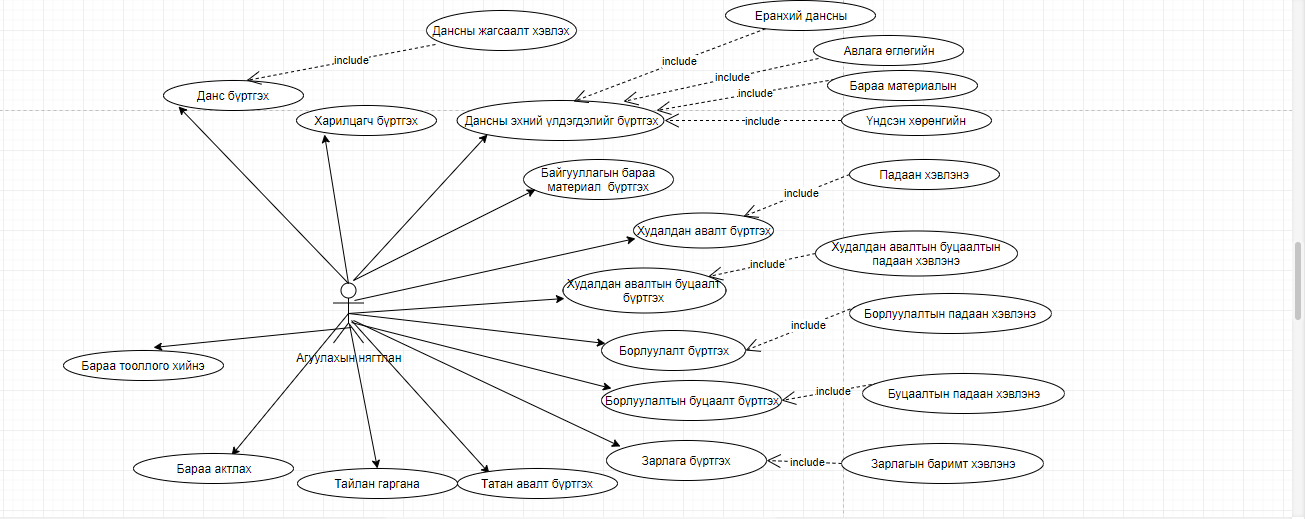
\includegraphics[width=14.5cm, height=17cm]{Diagrams/use1}
	\caption[Юзкэйс диаграм]{Юзкэйс диаграм}
	\label{text}
\end{figure}


\section{Юзкейс диаграмын тодорхойлолт}
\begin{center}
	\begin{table}[!htbp]
		\caption{Юзкейсийн тодорхойлолт: Худалдан авалт}
		\begin{tabular}{|p{4cm}|p{10cm}|}
			\hline
			Нэр: &   Худалдан авалт бүртгэх \\
			\hline
			ID: & 1 \\
			\hline
			Товч тайлбар: & Нягтлан системд шинээр худалдан авалт үүсгэнэ. \\
			\hline
			Триггер: & Нягтлан нь худалдан авалт хйих шаардлагатай болсон. \\
			\hline
			Үндсэн оролцогч: & Нягтлан \\
			\hline
			Хоёрдогч оролцогч: & Байхгүй  \\
			\hline
			Өмнөх нөхцөл: &  Веб сервер ажиллагаатай байх\\
			\hline
			Ажлын урсгал: & \begin{enumerate}
				\item Нягтлан нь худалдан авалт бүртгүүлэхийг сонгосноор энэ юз кейс эхлэнэ. 
				\item Систем нь худалдан авалт бүртгүүлэх цонхыг харуулна. 
				\item Нягтлан нь худалдан авалтын мэдээллийг (баримтын дугаар, эхлэх огноо, дуусах огноо, харилцагч, бараа код, нэр, тоо ширхэг, нэгж үнэ, нийт дүн) оруулна. 
				\item Веб сервер нь хэрэглэгчийн оруулсан мэдээллийг хадгална. 
				
				
			\end{enumerate}
			\\					  \hline
			Дараах нөхцөл: &
			\begin{enumerate}
				\item Нятлан худалдан авалтийг бүртгэж баримт хэвлэсэн байна. 
				\item Худалдан авалтын мэдээлэл баазад хадгалагдсан байна. 
			\end{enumerate}	   
			\\				   \hline
			Альтернатив урсгал: &  \begin{enumerate}
				\item Нягтлан худалдан авалтын бүртгэлийг цуцалсан.
				\item Веб сервер дээр алдаа гарсан. 
			\end{enumerate}
			\\	\hline
		\end{tabular}
	\end{table}
\end{center}

\vspace*{1in}
\begin{center}
	\begin{table}[!htbp]
		\caption{Юзкейсийн тодорхойлолт: Борлуулалт}
		\begin{tabular}{|p{4cm}|p{10cm}|}
			\hline
			Нэр: & Борлуулалт хийх  \\
			\hline
			ID: & 2 \\
			\hline
			Товч тайлбар: & Агуулахын нягтлан системд шинэ борлуулалт бүртгэнэ.  \\
			\hline
			Триггер: & Нягтлан системд борлуулалт нэмэхийг хүссэн. \\
			\hline
			Үндсэн оролцогч: & Нягтлан \\
			\hline
			Хоёрдогч оролцогч: & Веб  \\
			\hline
			Өмнөх нөхцөл: &  \begin{enumerate}
				\item Нягтлан өөрийн эрхээрээ нэвтэрсэн байх.
				\item Веб сервер ажиллагаатай байх.
			\end{enumerate}
			\\			\hline
			Ажлын урсгал: & \begin{enumerate}
				\item Нягтлан борлуулалт бүртгэхийг  сонгосноор энэ юз кейс эхлэнэ.
				\item Веб нь борлуулалт бүртгэх хуудсыг хэрэглэгчид харуулна.
				\item Нягтлан нь худалдан авалтын мэдээллийг (баримтын дугаар, эхлэх огноо, дуусах огноо, харилцагч, бараа код, нэр, тоо ширхэг, нэгж үнэ, нийт дүн) оруулна. 
				\item Борлуулалтын баримт хэвлэнэ.
				
				
				
			\end{enumerate}
			\\						\hline
			Дараах нөхцөл: & Сервер нь нягтлангийн оруулсан мэдээллийг хадгална. 
			Баримт хэвлэнэ\\
			\hline
			Альтернатив урсгал: & Серверийн өгөгдлийн сангын багтаамж дүүрсэн. \\
			\hline
		\end{tabular}
	\end{table}
\end{center}
\begin{center}
	\begin{table}[!htbp]
		\caption{Худалдан авсан бүтээгдэхүүний жагсаалтыг харах}
		\begin{tabular}{|p{4cm}|p{10cm}|}
			\hline
			Нэр: & Худалдан авсан бараа бүтээгдэхүүнийг харах  \\
			\hline
			ID: & 5 \\
			\hline
			Товч тайлбар: & Нягтлан худалдан авсан бараа бүтээгдэхүүний жагсаалтыг харна.  \\
			\hline
			Үндсэн оролцогч: & Нягтлан \\
			\hline
			Хоёрдогч оролцогч: & Байхгүй  \\
			\hline
			Өмнөх нөхцөл: &  Вебд нэвтэрсэн байх \\
			\hline
			Ажлын урсгал: &  \begin{enumerate}
				\item Нягтлан вэбд худалдан авсан бүтээгдэхүүнүүдийг харах зорилготой нэвтэрсэнээр энэ юзкейс эхэлнэ.
				\item Худалдан авсан бараа бүтээгдэхүүний жагсаалтыг харуулна. 
			\end{enumerate}	 \\
			\hline
			Дараах нөхцөл: & Нягтлан худалдан авсан бүтээгдэхүүний жагсаалтыг  харсан байна \\
			\hline 
			Альтернатив урсгал: & Байхгүй \\
			\hline
		\end{tabular}
	\end{table}
\end{center}

\begin{center}
	\begin{table}[!htbp]
		\caption{Бараа бүтээгдэхүүний хайлт хийх} 
		\begin{tabular}{|p{4cm}|p{10cm}|}
			\hline
			Нэр: & Хайлт хийх  \\
			\hline
			ID: & 7 \\
			\hline
			Товч тайлбар: & Нягтлан бараа бүтээгдэхүүний хайлт хийнэ.  \\
			\hline
			Үндсэн оролцогч: & Нягтлан \\
			\hline
			Хоёрдогч оролцогч: & Байхгүй  \\
			\hline
			Өмнөх нөхцөл: &  Вебд нэвтэрсэн байх \\
			\hline
			Ажлын урсгал: & \begin{enumerate}
				\item Нягтлан үндсэн хөрөнгө хэсгийг  сонгосоноор энэхүү юзкейс эхэлнэ.
				\item Веб хайлт хийх төрлүүдийг харуулна харуулна
				\item Нягтлан хайлт хийх төрөлөө сонгоно
				\item Веб нягтлангийн сонгосон хайлт хийх хэсгийг харуулна
				\item Нягтлан хайлтын утгаа оруулна
				\item IF(Хайлтын утга алдаатай бол)
				\begin{enumerate}
					\item[6.1] Веб хайлтын утга алдаатайг зочинд мэдэгдэнэ.
					\item[6.2] Веб нягтланд зөв хайлтын жишээ утга харуулна
				\end{enumerate}	
				\item ELSE IF(Таны хайсан утга )
				\begin{enumerate}
					\item[7.1] Веб таны хайсан утга илэрцгүй 
				\end{enumerate}
				\item Нягтланд хайлтанд илэрсэн утгуудыг харуулна
			\end{enumerate} 	\\
			\hline
			Дараах нөхцөл: & Нягтлан вебээс хүссэн хайлтаа олсон байна. \\
			\hline
			Альтернатив урсгал: & Нягтлангийн хайлт илэрцгүй байна.\\
			\hline
		\end{tabular}
	\end{table}
\end{center}



